% ---------------------------------------------------------------------------------------
% ---------------------------------------------------------------------------------------
% Specifications
% ---------------------------------------------------------------------------------------
% ---------------------------------------------------------------------------------------

\documentclass[12pt]{article}
\usepackage[letterpaper, margin=1in]{geometry}
\usepackage{newtxtext,newtxmath}
\usepackage[math-style=ISO]{unicode-math}
\usepackage{fullpage}
\usepackage[authoryear,sectionbib]{natbib}
\linespread{1.7}
\usepackage[utf8]{inputenc}
\usepackage{lineno}
\usepackage{titlesec}
\titleformat{\section}[block]{\Large\bfseries\filcenter}{\thesection}{1em}{}
\titleformat{\subsection}[block]{\Large\itshape\filcenter}{\thesubsection}{1em}{}
\titleformat{\subsubsection}[block]{\large\itshape}{\thesubsubsection}{1em}{}
\titleformat{\paragraph}[runin]{\itshape}{\theparagraph}{1em}{}[. ]
\renewcommand{\refname}{Literature Cited}
\DeclareTextSymbolDefault{\dh}{T1}
\medmuskip=8mu 
\thickmuskip=10mu
\usepackage{graphicx}
\usepackage{booktabs}
\renewcommand{\thetable}{\Roman{table}}
\usepackage{caption}
\captionsetup{justification = raggedright,
              singlelinecheck = false,
              labelfont = bf}






% ---------------------------------------------------------------------------------------
% ---------------------------------------------------------------------------------------
% Title page
% ---------------------------------------------------------------------------------------
% ---------------------------------------------------------------------------------------

\title{Photosynthesis-light relationships are more variable in time than in space 
        for a shallow eutrophic lake}

\author{
Joseph S. Phillips$^{1,2,\dagger}$ \\
Amanda R. McCormick$^{1,3}$ \\
Jamieson C. Botsch$^{1}$ \\
Kristian R. Book$^{1}$ \\
Anthony R. Ives$^{1}$}

\usepackage{amsmath} % for split math environment

\date{}

\begin{document}

\raggedright
\setlength\parindent{0.25in}

\maketitle

\noindent{} 1. Department of Integrative Biology, University of Wisconsin, Madison, Wisconsin 53706 USA

\noindent{} 2. Department of Aquaculture and Fish Biology, H\'{o}lar University, Skagafj\"{o}r{\dh}ur 551 Iceland

\noindent{} 3. Department of Land, Air and Water Resources, 
University of California, Davis, CA, USA

\noindent{} $\dagger$ E-mail: joseph@holar.is

\bigskip

Running head: {Variable PI curves}

\linenumbers{}

\clearpage





% ---------------------------------------------------------------------------------------
% ---------------------------------------------------------------------------------------
% Abstract
% ---------------------------------------------------------------------------------------
% ---------------------------------------------------------------------------------------


\section*{Abstract}





\bigskip

\textit{Keywords}: {}

\clearpage





% ---------------------------------------------------------------------------------------
% ---------------------------------------------------------------------------------------
% Introduction
% ---------------------------------------------------------------------------------------
% ---------------------------------------------------------------------------------------

\section*{Introduction}






% ---------------------------------------------------------------------------------------
% ---------------------------------------------------------------------------------------
% Methods
% ---------------------------------------------------------------------------------------
% ---------------------------------------------------------------------------------------




\section*{Methods}





% ---------------------------------------------------------------------------------------
% ---------------------------------------------------------------------------------------
% Results
% ---------------------------------------------------------------------------------------
% ---------------------------------------------------------------------------------------



\section*{Results}







% ---------------------------------------------------------------------------------------
% ---------------------------------------------------------------------------------------
% Discussion
% ---------------------------------------------------------------------------------------
% ---------------------------------------------------------------------------------------



\section*{Discussion}






% ---------------------------------------------------------------------------------------
% ---------------------------------------------------------------------------------------
% Acknowledgments
% ---------------------------------------------------------------------------------------
% ---------------------------------------------------------------------------------------

\section*{Acknowledgments}

This work was supported by National Science Foundation grants 
DEB-1052160, DEB-1556208 to Anthony R. Ives,
and Graduate Research Fellowships DGE-1256259 and DGE-1747503.
The M\'{y}vatn Research Station directed by \'{A}rni Einarsson
provided logistical and scientific support.
We thank Jill Welter for feedback on the experiments
and numerous research interns for for assistance with fieldwork.

% ---------------------------------------------------------------------------------------
% ---------------------------------------------------------------------------------------
% Literature Cited
% ---------------------------------------------------------------------------------------
% ---------------------------------------------------------------------------------------



\bibliographystyle{ecology.bst}
\clearpage

\bibliography{refs.bib}

\clearpage





% ---------------------------------------------------------------------------------------
% ---------------------------------------------------------------------------------------
% Tables & Figures
% ---------------------------------------------------------------------------------------
% ---------------------------------------------------------------------------------------

% ---------------------------------------------------------------------------------------
% Captions
% ---------------------------------------------------------------------------------------


% ---------------------------------------------------------------------------------------
% NEP
% ---------------------------------------------------------------------------------------

\begin{figure}
\centering
\linespread{1}
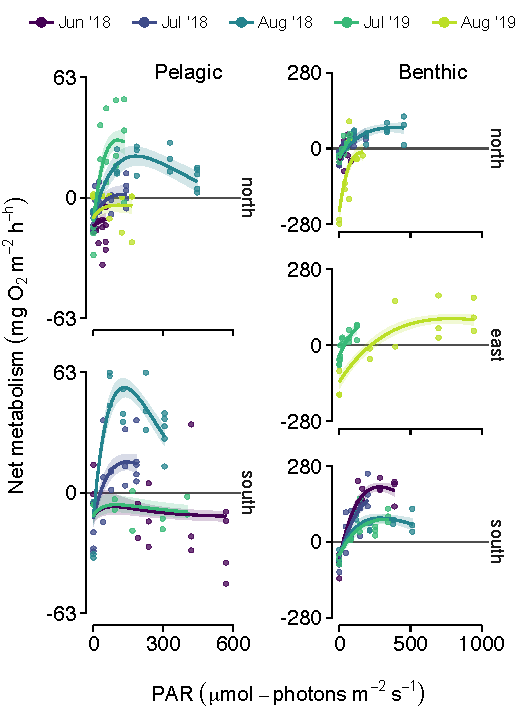
\includegraphics{../analysis/figures/fig_nep.pdf}
\caption{\label{fig:nep}
Caption.
}
\end{figure}

\clearpage



% ---------------------------------------------------------------------------------------
% SD
% ---------------------------------------------------------------------------------------

\begin{figure}
\centering
\linespread{1}
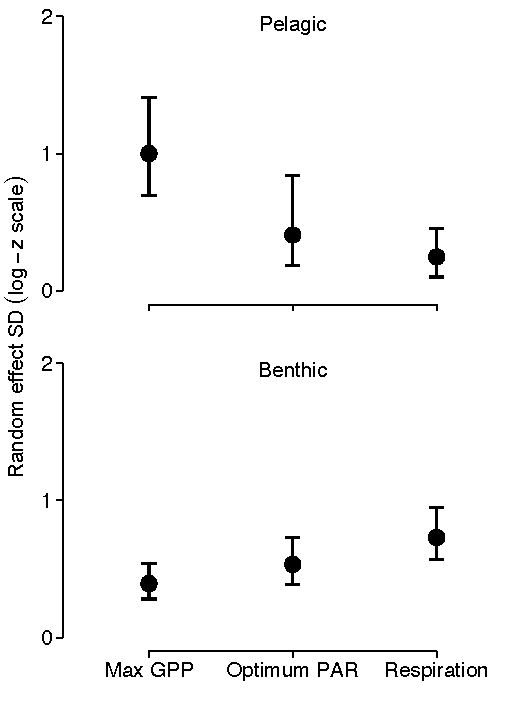
\includegraphics{../analysis/figures/fig_sd.pdf}
\caption{\label{fig:sd}
Caption.
}
\end{figure}

\clearpage

% ---------------------------------------------------------------------------------------
% PAR
% ---------------------------------------------------------------------------------------

\begin{figure}
\centering
\linespread{1}
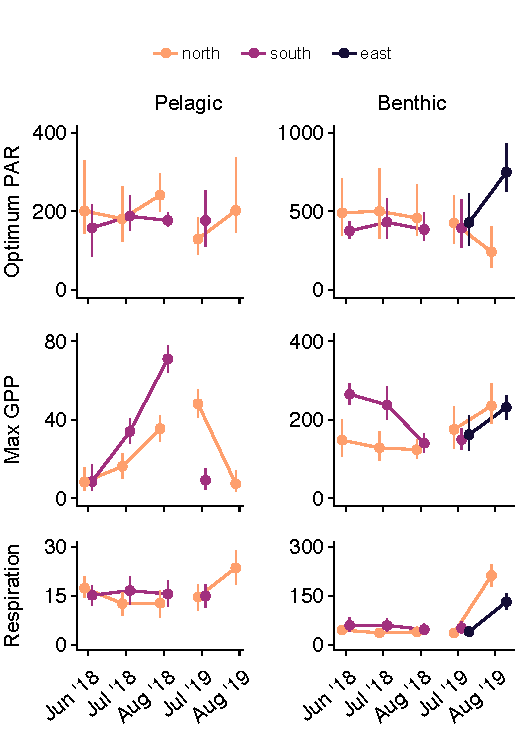
\includegraphics{../analysis/figures/fig_par.pdf}
\caption{\label{fig:par}
Caption. 
}
\end{figure}

\clearpage

% ---------------------------------------------------------------------------------------
% VAR
% ---------------------------------------------------------------------------------------

\begin{figure}
\centering
\linespread{1}
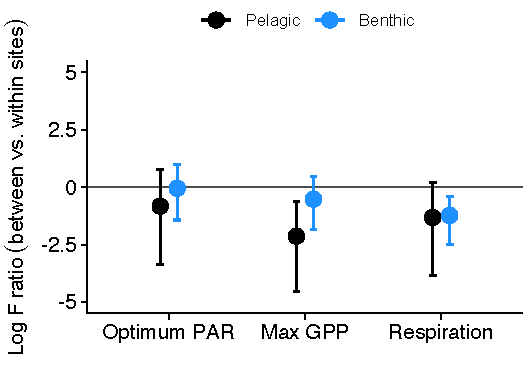
\includegraphics{../analysis/figures/fig_var.pdf}
\caption{\label{fig:var}
Caption. 
}
\end{figure}

\clearpage



% ---------------------------------------------------------------------------------------
% ---------------------------------------------------------------------------------------
% Supplement
% ---------------------------------------------------------------------------------------
% ---------------------------------------------------------------------------------------

\renewcommand{\thefigure}{S\arabic{figure}}
\renewcommand{\theequation}{S\arabic{equation}}
\renewcommand{\thetable}{S\arabic{table}}
\setcounter{equation}{0}
\setcounter{figure}{0}
\setcounter{table}{0}


\end{document}
